\documentclass[border=1pt]{standalone}
\usepackage{tikz}
\usetikzlibrary{arrows.meta,calc}

\begin{document}
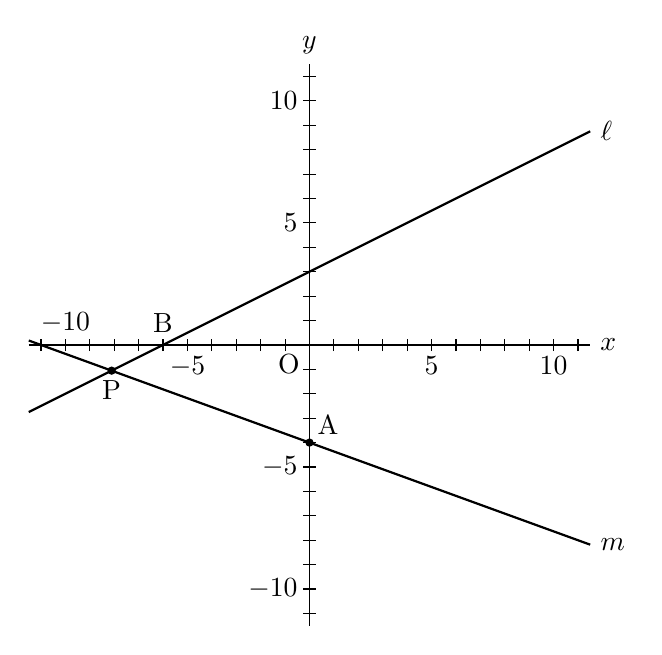
\begin{tikzpicture}[x=3.1mm, y=3.1mm]

    \pgfmathsetmacro{\xmax}{11.5}
    \pgfmathsetmacro{\ymax}{11.5}


    \pgfmathsetmacro{\d}{0.25}

    % 座標軸
    \draw[semithick] (-\xmax,0) -- (\xmax,0) node[right] {$x$};
    \draw[semithick] (0,-\ymax) -- (0,\ymax) node[above] {$y$};
    
    % x軸・y軸の目盛り
    \foreach \x in {-11,-10,...,11} {
        \draw (\x,-\d) -- (\x,\d);
    }
    \foreach \y in {-11,-10,...,11} {
        \draw (-\d,\y) -- (\d,\y);
    }
    \foreach \x in {-5,5,10} {
        \node[below, outer sep=1pt] at (\x,0) {$\x$};
    }
    \foreach \y in {-10,-5,5,10} {
        \node[left, outer sep=1pt] at (0,\y) {$\y$};
    }
    \node at (-10,0) [above, outer sep=1pt] {$-10$};


    % 直線 l: y = (1/2)x + 3 と 直線 m: y = (-4/11)x - 4 を描画
    \draw[thick] (-\xmax,{-\xmax/2+3}) -- (\xmax,{\xmax/2+3}) node[right] {$\ell$};
    \draw[thick] (-\xmax,{4*\xmax/11-4}) -- (\xmax,{-4*\xmax/11-4}) node[right] {$m$};

    % 原点
    \node[below left] at (0,0) {$\mathrm{O}$};
    
    % 点 A(0, -4)
    \fill (0,-4) circle (1.5pt) node[above right, outer sep=-.4pt] {$\mathrm{A}$};
    
    % 点 B(-6, 0)
    \node[above, outer sep=1pt] at (-6,0) {$\mathrm{B}$};
    
    % 点 P
    \fill (-154/19,-20/19) circle (1.5pt) node[below] {$\mathrm{P}$};
    
    
\end{tikzpicture}
\end{document}
